%% Roman Link's personalized LaTeX Beamer template 
%% contact: rlink@gwdg.de

%% define document class and settings -----------------------------------
\documentclass[usepdftitle=false]{beamer}

%% fonts and input encoding ---------------------------------------------
\usepackage[T1]{fontenc}
\usepackage[utf8x]{inputenc}
\usepackage{lmodern}

%% language support -----------------------------------------------------
\usepackage[english]{babel} % english hyphenation etc.
\usepackage{babelbib}       % multi-language references

%% graphics and colors --------------------------------------------------
\usepackage{graphicx}  
\usepackage{color,pgf}
\usepackage{pdfpages}  % enables the use of pdf graphics

%% mathematical symbols  ------------------------------------------------
\usepackage{amsmath, amsfonts, amssymb, pgf}
\usepackage{eulervm}

%% references with natbib -----------------------------------------------
%\usepackage[round]{natbib}
%\def\newblock{} % hilft gegen absurde fehler mit natbib

%% tweaks of appearance -------------------------------------------------
\usepackage{subscript} % subscripts outside of math expressions
\usepackage{booktabs}  % better-looking tables
\usepackage{ragged2e}  % justified text in Beamer documents with  	
                       % \justifying{}
\usepackage{setspace}  % control line space with spacing environment

%% LaTeX Beamer settings ------------------------------------------------
\mode<presentation>{
	\usecolortheme{seahorse,rose}
	\useinnertheme[shadow]{rounded}
	% \useoutertheme[hideothersubsections,right,width=4em,frame  number]{sidebar}
	% \useoutertheme{infolines}
	% \useoutertheme{split}
	\useoutertheme[subsection=false,footline=authortitle]{miniframes}
	\setbeamercovered{transparent}
}

%% add slide numbers to all slides --------------------------------------
\addtobeamertemplate{navigation symbols}{
  {\usebeamercolor{section in toc}
   \footnotesize
   \insertframenumber/\inserttotalframenumber}
   \hspace{48em}
}{}

%% changes of beamer fonts ----------------------------------------------
\setbeamerfont{section in toc}{size=\normalsize,series=\bfseries}
\setbeamerfont{title}{series=\bfseries}
\setbeamerfont{frametitle}{size=\Large,series=\bfseries}

%% new LaTeX commands ---------------------------------------------------
\newcommand{\sub}[1]{\textsubscript{#1}}
\newcommand{\Sup}[1]{\textsuperscript{#1}}
\newcommand{\COO}{CO\textsubscript{2}}
\newcommand{\masl}{m~a.s.l.}
\newcommand{\gc}{$^{\circ}$C}
\newcommand{\tilt}{$\sim$}
\newcommand{\blue}[1]{{\color{blue!50!black}#1}}
\newcommand{\Blue}[1]{{\color{blue!50!black}\textbf{#1}}}
\newcommand{\eg}{e.\,g.}
\newcommand{\Eg}{E.\,g.}
\newcommand{\rar}{$\rightarrow$}
\newcommand{\lar}{$\leftarrow$}
\newcommand{\Rar}{$\Rightarrow$}
\newcommand{\Lar}{$\Leftarrow$}
\newcommand{\source}[1]{\baselineskip8pt{\tiny \color{gray} #1}}
\newcommand{\tw}{\textwidth}
\newcommand{\ddx}[2]{
	\frac{\mathrm{d}}{\mathrm{d}#2}#1 
	}
\newcommand{\ddxx}[2]{
	\frac{\mathrm{d^2}}{\mathrm{d}#2^2}#1
	}
\newcommand{\code}[1]{
	{\footnotesize 
	 \color{blue}
   \texttt{#1}}
   \normalsize
   \color{black}
  }

%% new environment for slides with changed margins ----------------------
\newenvironment{changemargin}[2]{%
	\begin{list}{}{%
			\setlength{\topsep}{0pt}%
			\setlength{\leftmargin}{#1}%
			\setlength{\rightmargin}{#2}%
			\setlength{\listparindent}{\parindent}%
			\setlength{\itemindent}{\parindent}%
			\setlength{\parsep}{\parskip}%
		}%
		{\item[]}
	\end{list}
}

%% pdf information  -----------------------------------------------------
\hypersetup{
	pdfauthor={Roman M. Link},
	pdftitle={Drought in tropical forests},
}

%% title page settings --------------------------------------------------
\title{Drought in tropical forests}
\subtitle{\normalfont The role of tree height and wood density for hydraulic efficiency, productivity and vulnerability to cavitation of trees along a lowland precipitation gradient}
\author[R. Link]{Roman Link}
\date{January 25, 2018}
\institute[University of Göttingen]{
Department of Plant Ecology and Ecosystem Research\\ Georg August University of Göttingen}
%\titlegraphic{ \vspace*{2em}
%\includegraphics[width=0.7\textwidth]{logouni.png}}
% logo - shown on all pages
\logo{
\includegraphics[width=20em]{logo_uni_goe_transparent.png}}

%% start of document ----------------------------------------------------
\begin{document}

%% insert title page ----------------------------------------------------
\begin{frame}
\titlepage
\end{frame}

%% begin of regular slides ----------------------------------------------
\begin{frame}
	\frametitle{Structure of my PhD project}
	\begin{itemize}
		\item \Blue{Chapter 1:} Predicting radial sap flow profiles from Costa Rican tropical dry forest species
		\item \Blue{Chapter 2:} Predicting plant vulnerability to embolism in Costa Rican humid tropical forest species
		\item \Blue{Chapter 3:} Relationship between productivity, structural and functional, wood anatomical and hydraulic traits of tropical forest species from Costa Rica
		\item<visible@2> \Blue{Bonus Chapter:} Maximum-likelihood estimation of xylem vessel lengths
    \end{itemize}	
\end{frame}

\begin{frame}
	\frametitle{Structure of this presentation}
	\begin{enumerate}
		\item Introduction
		\item Predicting radial sap flow profiles from Costa Rican tropical dry forest species
		\item Predicting plant vulnerability to embolism in Costa Rican humid tropical forest species
		\item Relationship between productivity, structural and functional, wood anatomical and hydraulic traits of tropical forest species from Costa Rica
		\item<visible@2| alert@2> Maximum-likelihood estimation of xylem vessel lengths: \textbf{Not in the focus of this presentation!}
	\end{enumerate}	
\end{frame}

\section{Introduction}
\begin{frame}
	\frametitle{Introduction}
	\begin{itemize}
		\item Basics about plant water relations
		\item Why is it important to know about drought effects in the tropics?
	\end{itemize}
\end{frame}

\begin{frame}
	\frametitle{Main research questions}
	\begin{itemize}
		\item This one's gonna be tough
	\end{itemize}
\end{frame}

\begin{frame}
	\frametitle{Design of the study}
	\begin{minipage}{0.5\tw}
		\begin{itemize}
			\item 5 research sites along a rainfall gradient on the Pacific shoreline of Costa Rica 			
			\item Gradient from tropical dry forest to humid tropical lowland forest
			\item Based on existing research sites of the \Blue{Instituto Tecnológico de Costa Rica}
		\end{itemize}		
	\end{minipage}
	\begin{minipage}{0.48\tw}
		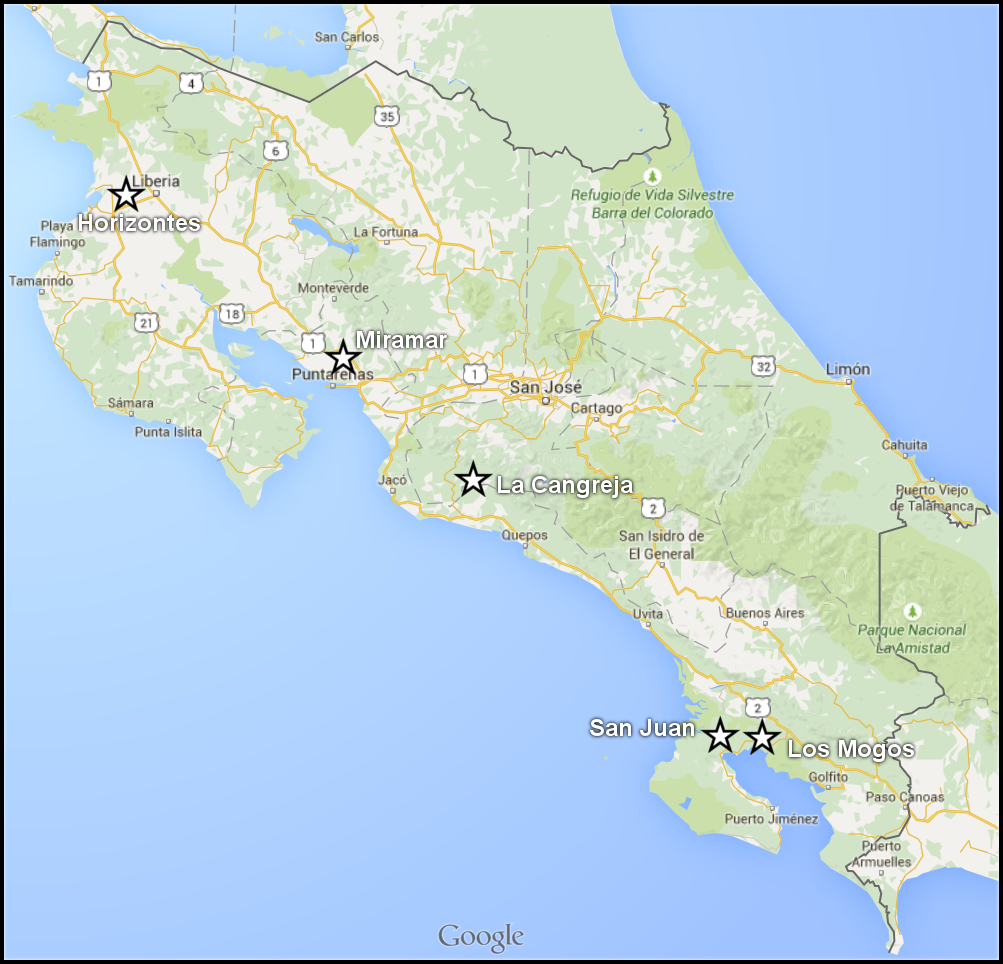
\includegraphics[width = \tw]{figures/map_01_all_sites.png}  	
	\end{minipage}
\end{frame}

\begin{frame}
	\frametitle{Design of the study}
\begin{itemize}
	\item At each of the 5 research sites:
	\begin{itemize}
		\item 8 species representing a gradient in tree height and wood density
		\item 5 replicates per species
		\item[\Rar] 40 trees per site, 200 trees in total
	\end{itemize}
	\item Field measurements of temperature, relative humidity and precipitation
\end{itemize}
\end{frame}

\begin{frame}
	\frametitle{Problems with the design}
	\begin{itemize}
		\item Opportunistic use of pre-existing plots
		\item Different plot sizes and numbers at each site
		\item Differences in historic land use (pristine primary forest vs. disturbed primary forest vs. secondary forest)
		\item[\rar] Plot-based comparisons are difficult
		\item[\Rar] Not that important for our (eco-physiological) research questions, but limits usability of plot network for other studies
	\end{itemize}
\end{frame}


\section{Radial sap flow profiles}
\begin{frame}
	\frametitle{First chapter: radial sap flow profiles}
	\begin{minipage}{0.5\tw}
	 \textbf{Sap flow measurements:}
	 \begin{itemize}
	 	\item<+-| alert@+> Practical limitations \rar\ only in dry forest (Horizontes)
	 	\item<+-| alert@+> 4 measurement campaigns of $\pm$ 1 week during rainy season of 2015
	 	\item<+-| alert@+> 40 trees of 8 species	
	 	\item<+-| alert@+> measured with the Heat Field Deformation (HFD) method			
	 \end{itemize}			
	\end{minipage}
	\begin{minipage}{0.48\tw}
		\only<1-3>{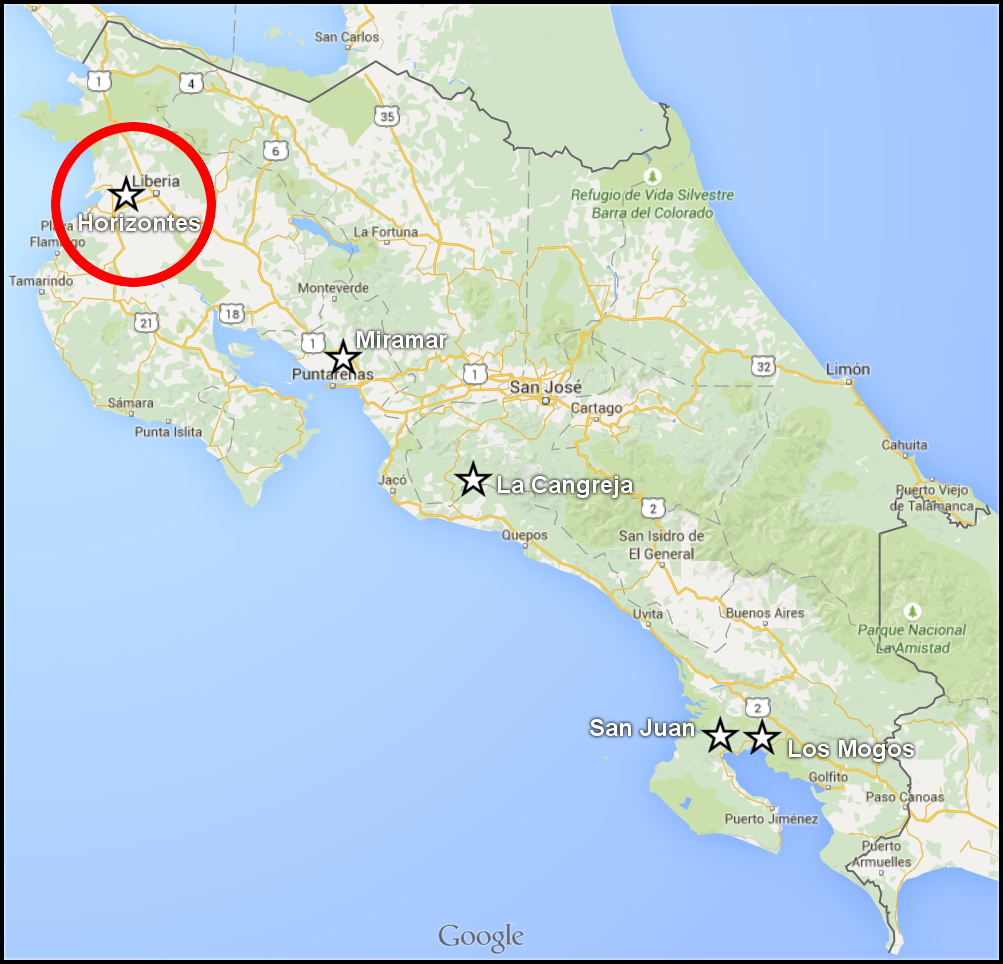
\includegraphics[width = \tw]{figures/map_02_horizontes.png}} 	
		\only<4>{\includegraphics[width = 0.75\tw]{figures/HFD_01_sensor.JPG}}
	\end{minipage}
\end{frame}

\begin{frame}
	\frametitle{Heat field deformation sensors}
	\begin{minipage}{0.5\tw}
		\textbf{Working principle:}
		\begin{itemize}
			\item<+-| alert@+> 1 heater and 3 temperature sensors inserted into wood
			\item<+-| alert@+> Heater heats constantly with known caloric input
			\item<+-| alert@+> Sap movement \rar\ faster heat transport in flow direction
			\item<+-| alert@+> Temperature differences between sensors are used for estimation of sap flux density at different depths
		\end{itemize}						
	\end{minipage}
	\begin{minipage}{0.48\tw}
			\only<1-2>{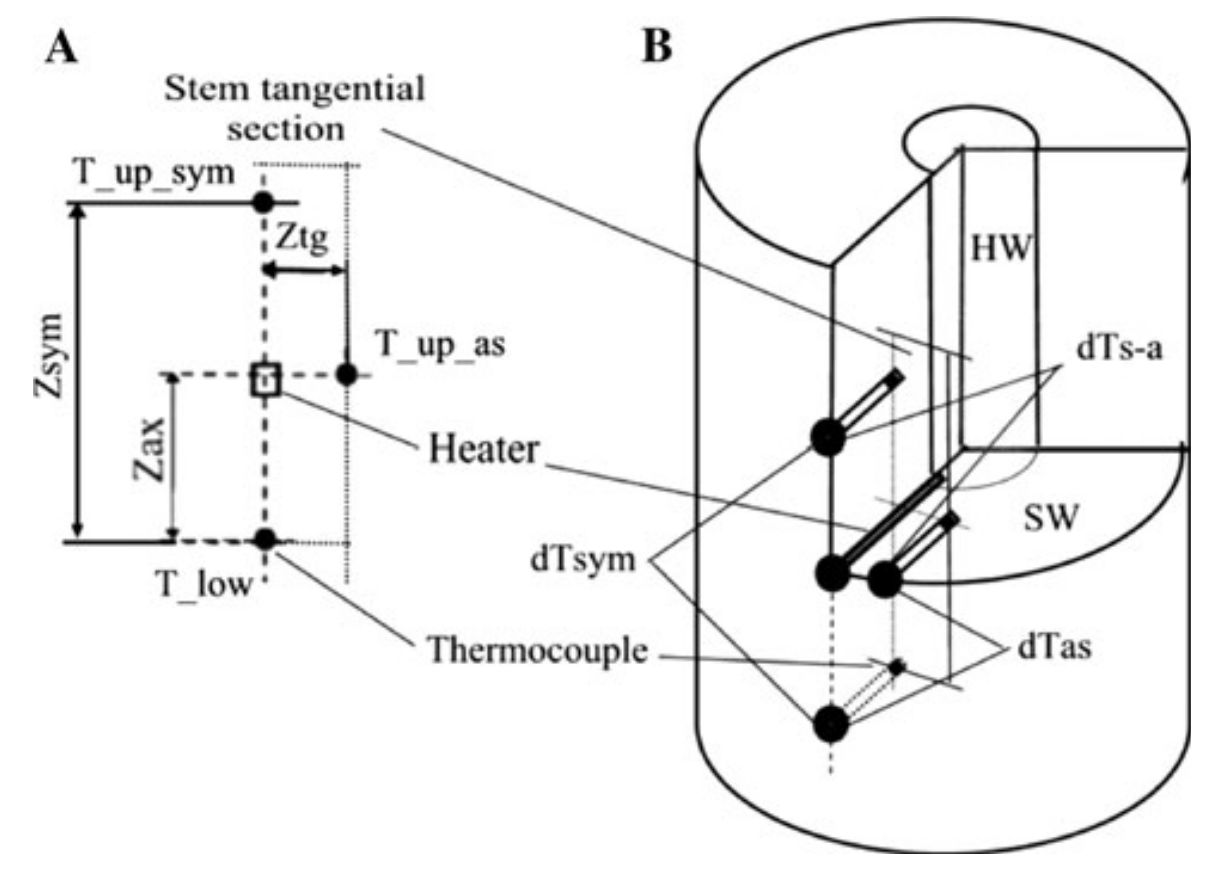
\includegraphics[width = \tw]{figures/nadezhdina_01.png}}
			\only<3-4>{\quad\quad 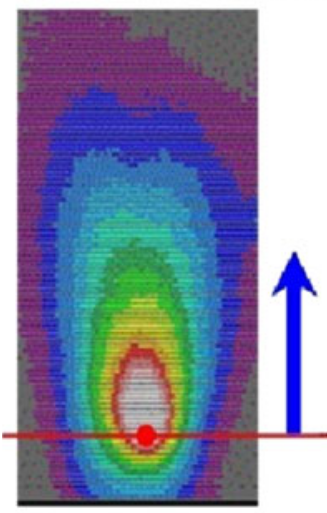
\includegraphics[width = 0.6\tw]{figures/nadezhdina_02.png}}\\
				
				\source{Image source: Nadezhdina et al., 2012}
	\end{minipage}
\end{frame}

\begin{frame}[t]
	\frametitle{Heat field deformation sensors}
	\begin{itemize}
		\item<only@1| alert@1> Original idea: Comparison of sap flow and plant water use between species with different trait combinations
		\item<only@2-> Problem: newer research indicates that
		\begin{itemize}
			\item[a)]<2-| alert@2> The mechanistic explanation of the HFD method (Nadezhdina et al., 2012) is flawed (Vandegehuchte et al., 2012)\\ \rar\ species-specific calibration likely necessary in most cases
			\item[b)]<3-| alert@3> Calibration parameters are not consistent within species (Fuchs et al., 2017)
		\end{itemize}	
		\item<only@4-| alert@4> Relative values are probably reliable, absolute values have to be handled with care
		\item<only@5| alert@5>[\Rar] \textbf{Decision for analysis: focus on radial gradients of sap flux}
	\end{itemize}
	\only<2>{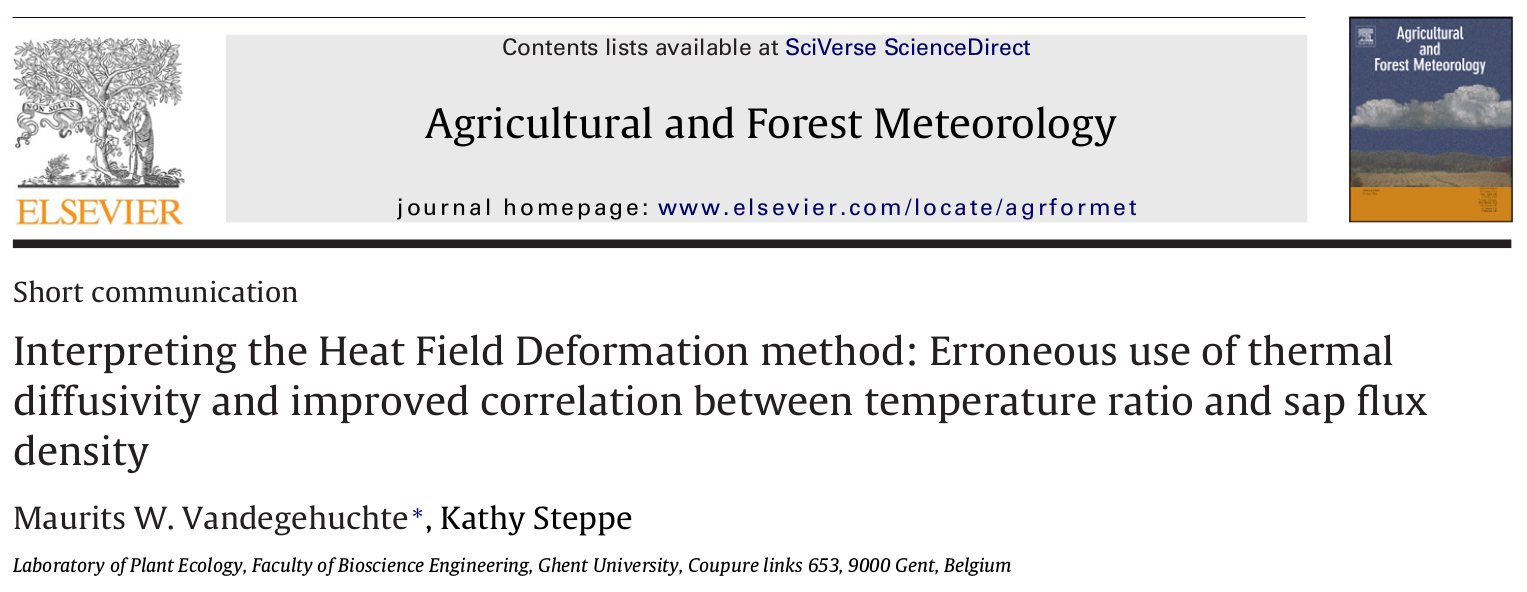
\includegraphics[width = \tw]{figures/vandegehuchte_01.png}}
  \only<3>{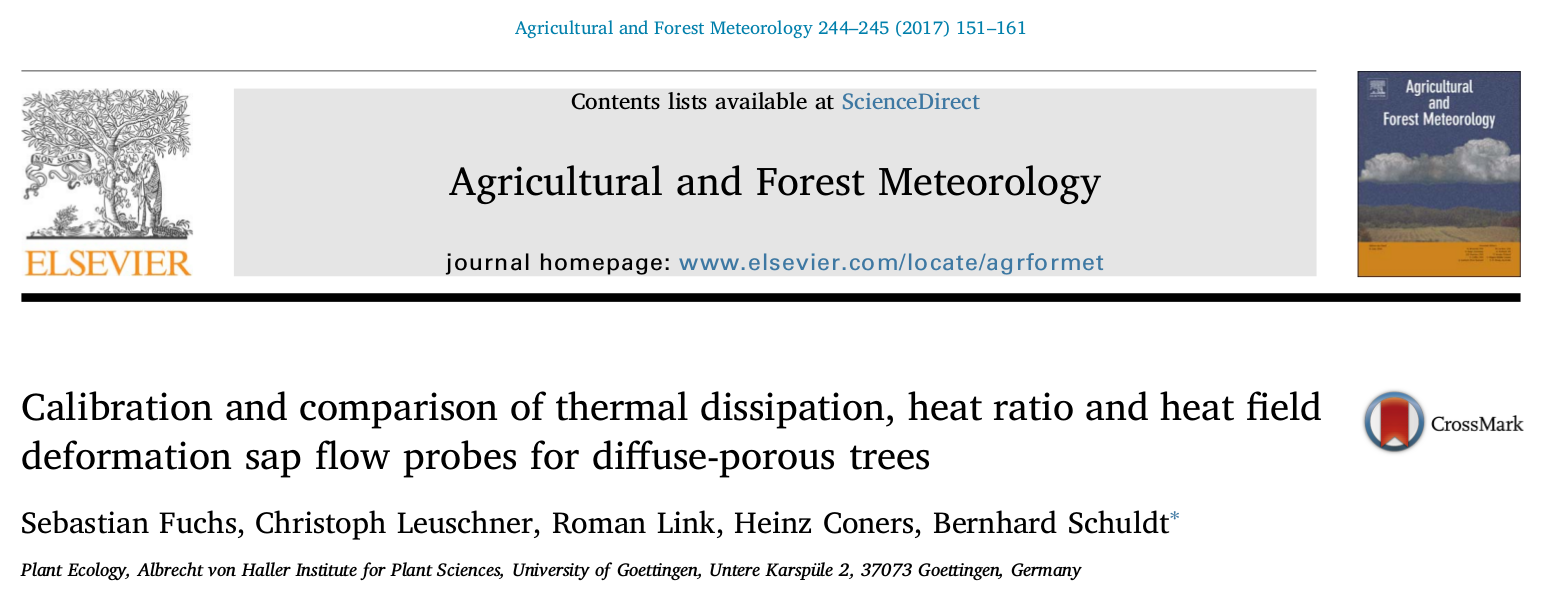
\includegraphics[width = \tw]{figures/HFDSeb_01_paper.png}}	
\end{frame}

\begin{frame}
	\frametitle{Research questions \& hypotheses}
	\begin{minipage}{0.38\tw}
		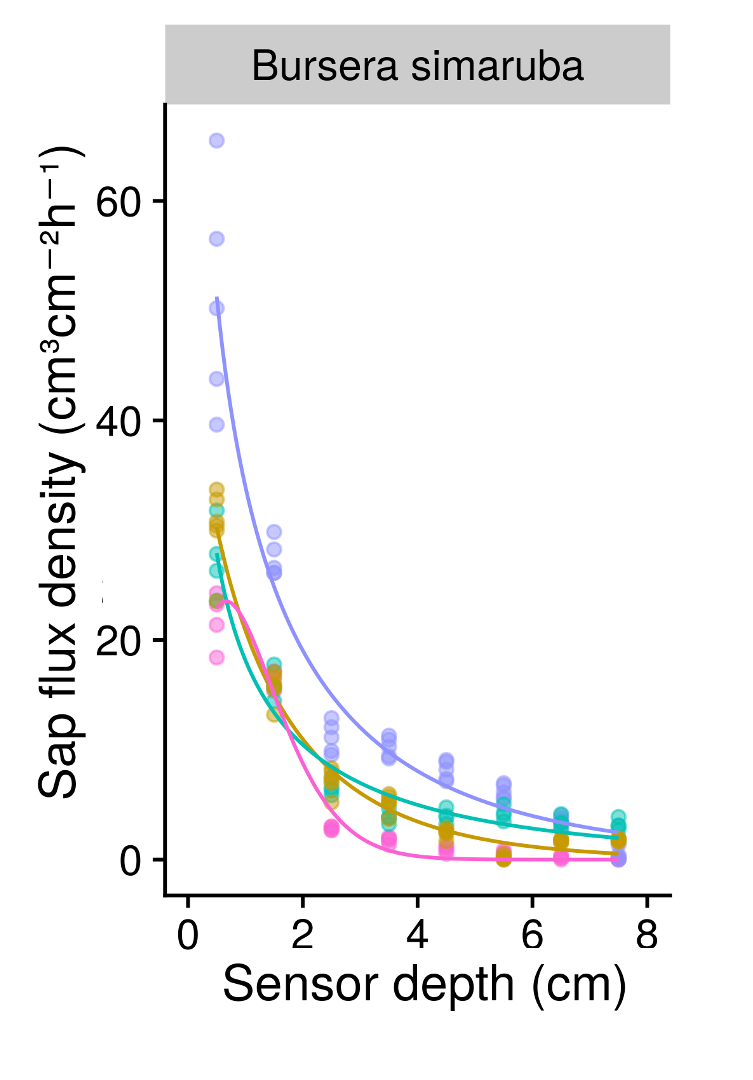
\includegraphics[width = \tw]{figures/HFD_05_profile_simarouba.png}
	\end{minipage}
	\begin{minipage}{0.6\tw}
			\begin{itemize}[<+-| alert@+>]
			\item For studies of water use radial gradients in sap flow are very important, but only few methods take it into account	
			\item Species specific measurements are problematic in the tropics		
			\item[\Rar] \Blue{Question:} Is it possible to predict the shape of the radial sap flow profile based on tree traits?
			\item<visible@+| alert@+>[\Rar] \Blue{Hypothesis:} The shape of the radial sap flow profile is related to \textbf{wood density} and \textbf{tree height}
		\end{itemize}						
	\end{minipage}

\end{frame}

\begin{frame}
	\frametitle{Data analysis}
	\begin{itemize}
		\item Non-linear Bayesian hierarchical model
		\item Simultaneously estimating shape of profiles on one stage on the model, and regressing relationship between parameters and predictors on second model stage
		\item ONE SLIDE!
	\end{itemize}
\end{frame}

\begin{frame}
	\frametitle{Preliminary results I - predicted profiles}
	\begin{itemize}
		\item Figure and some explication 
	\end{itemize}
\end{frame}

\begin{frame}
	\frametitle{Preliminary results II - predicted relationships}
	\begin{itemize}
		\item Figure and some explication 
	\end{itemize}
\end{frame}

\section{Vulnerability curves}
\begin{frame}
	\frametitle{Vulnerability curves}
	\begin{itemize}
		\item What are vulnerability curves?
		\item What kind of information do they offer?
	\end{itemize}  
\end{frame}

\begin{frame}
	\frametitle{The Cavi1000}
	\begin{itemize}
		\item Some photos, basic information about how it works
	\end{itemize}
\end{frame}

\begin{frame}
	\frametitle{Research questions \& hypotheses}
	\begin{itemize}
		\item Plant vulnerability to embolism can be predicted by structural, functional and wood anatomical traits
	\end{itemize}
\end{frame}

\begin{frame}
	\frametitle{Data analysis}
	\begin{itemize}
		\item Non-linear Bayesian hierarchical model
		\item Compare to HFD model, mention Ogle et al. 2009
		\item ONE SLIDE!
	\end{itemize}
\end{frame}

\begin{frame}
	\frametitle{Observed vulnerability curves}
	\begin{itemize}
		\item Do not overinterprete!
	\end{itemize}
\end{frame}

\section{The big picture}
\begin{frame}
	\frametitle{Big picture}
	\begin{itemize}
		\item Analyzed variables (methods section)
		\item Design		
	\end{itemize}
\end{frame}

\begin{frame}
	\frametitle{Growth data}
	\begin{itemize}
		\item short description
		\item picture
	\end{itemize}
\end{frame}

\begin{frame}
	\frametitle{Wood anatomy}
	\begin{itemize}
		\item short description
		\item picture
	\end{itemize}
\end{frame}

\begin{frame}
	\frametitle{Non-structural carbohydrates}
	\begin{itemize}
		\item short description
		\item picture
		\item data not available so far
	\end{itemize}
\end{frame}

\begin{frame}
	\frametitle{Research questions \& hypotheses}
	\begin{itemize}
		\item Lots and lots of hypotheses
	\end{itemize}
\end{frame}

\begin{frame}
	\frametitle{Data analysis}
	\begin{itemize}
		\item Short explanation of structural equation models		
	\end{itemize}
\end{frame}

\begin{frame}
	\frametitle{Meta-model \& causal diagram}
	\begin{itemize}
		\item figures on one or two slides		
	\end{itemize}
\end{frame}

\begin{frame}
	\frametitle{Example for SEM: Martyna's paper}
	\begin{itemize}
		\item Meta-model, causal diagram \& final path model	
	\end{itemize}
\end{frame}

\begin{frame}
	\frametitle{Summary}
	\begin{itemize}
		\item Sap flow
		\item Vulnerability curves
		\item SEM
	\end{itemize}
\end{frame}


\begin{frame}
	\frametitle{Thanks \& goodbye}
	\begin{itemize}
		\item Names of assistants (pictures?)
	\end{itemize}
\end{frame}

\section{References}
\begin{frame}
	\frametitle{References}
	\begin{itemize}
		\item \textbf{Fuchs S, Leuschner C, Link R, Coners H, Schuldt B, 2017.}
		Calibration and comparison of thermal dissipation, heat ratio and heat field deformation sap flow probes for diffuse-porous trees,
		\textit{Agricultural and Forest Meteorology} \textbf{244–245},151-161. \url{https://doi.org/10.1016/j.agrformet.2017.04.003.}.
	\end{itemize}
\end{frame}
\end{document}
